\section{Nondeterministic Finite Automaton}
(( NOTE: SHARPEN UP SECTION TO A MORE PRECISE DEFINITION OF NFA))

\begin{mydef}
An nondeterministic finite automaton (NFA) consists of a finite set of states, $Q$, with a finite number of transitions, $T$, between them.

%$T$ is a relation behavior \begin{math}\end{math}

In $Q$ there's one starting state, and a subset of accepting (final) states.

Each transition in $T$ is a has a starting state, and a destination state, and is labeled either by a character, or by $\epsilon$, which indicates an epsilon-transition (empty transition).
\end{mydef}

\subsubsection{Conversion from RE to NFA}
One of the main reasons for using NFAs when working with regular expressions is the direct correlation between regular expressions and NFAs. Each expression can be converted to an NFA, and vice versa.
\\
(( NOTE: We'll include a table with conversions ))
\\
%With little effort every regular expression can be translated into a graph, which can then be analysed.

\begin{figure}[h!]
\begin{minipage}[b]{0.40\linewidth}
  \centering
      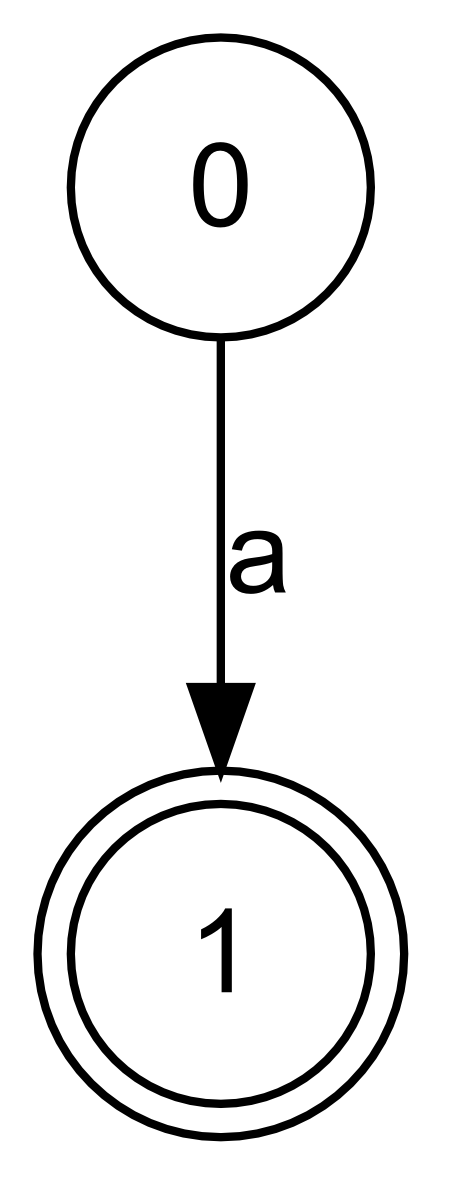
\includegraphics[width=0.2\textwidth]{lib/A.png}
  \caption{NFA of the expression $a$}
\label{fig:A}
  \end{minipage}
\begin{minipage}[b]{0.40\linewidth}

  \centering
      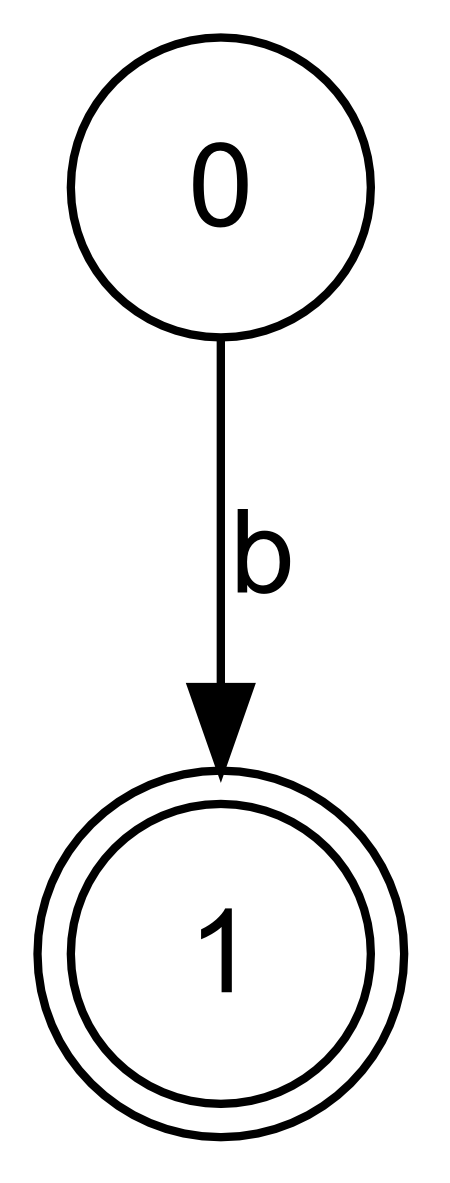
\includegraphics[width=0.2\textwidth]{lib/B.png}
  \caption{NFA of the expression $b$}
  \label{fig:B}

    \end{minipage}
\end{figure}


For example two NFAs of regular expression $a$ and $b$ will appear as shown in Figure~\ref{fig:A} \& \ref{fig:B}, each of them starts in node $0$ and ends in node $1$, and these nodes are connected by a one-way transition with a value $a$ or $b$. %, it may be worth noting that our implementation always converts to lower case when constructing and matching.

To construct the NFA for $A | B$ , one will first have to construct an NFA for both $A$ and $B$, which will then be combined, making the full NFA. The $|$ operator this is achieved by constructing two new nodes, the first having epsilon-transition pointing to the start node of each of the two NFAs $A$ and $B$, then for each NFA $A$ and $B$ the ending node will instead of ending the NFA, have a new epsilon-transition to the second new node, in the figure below, Figure~\ref{fig:A_OR_B}, the two new nodes are labeled $0$ and $5$:

\begin{figure}[h!]
  \centering
      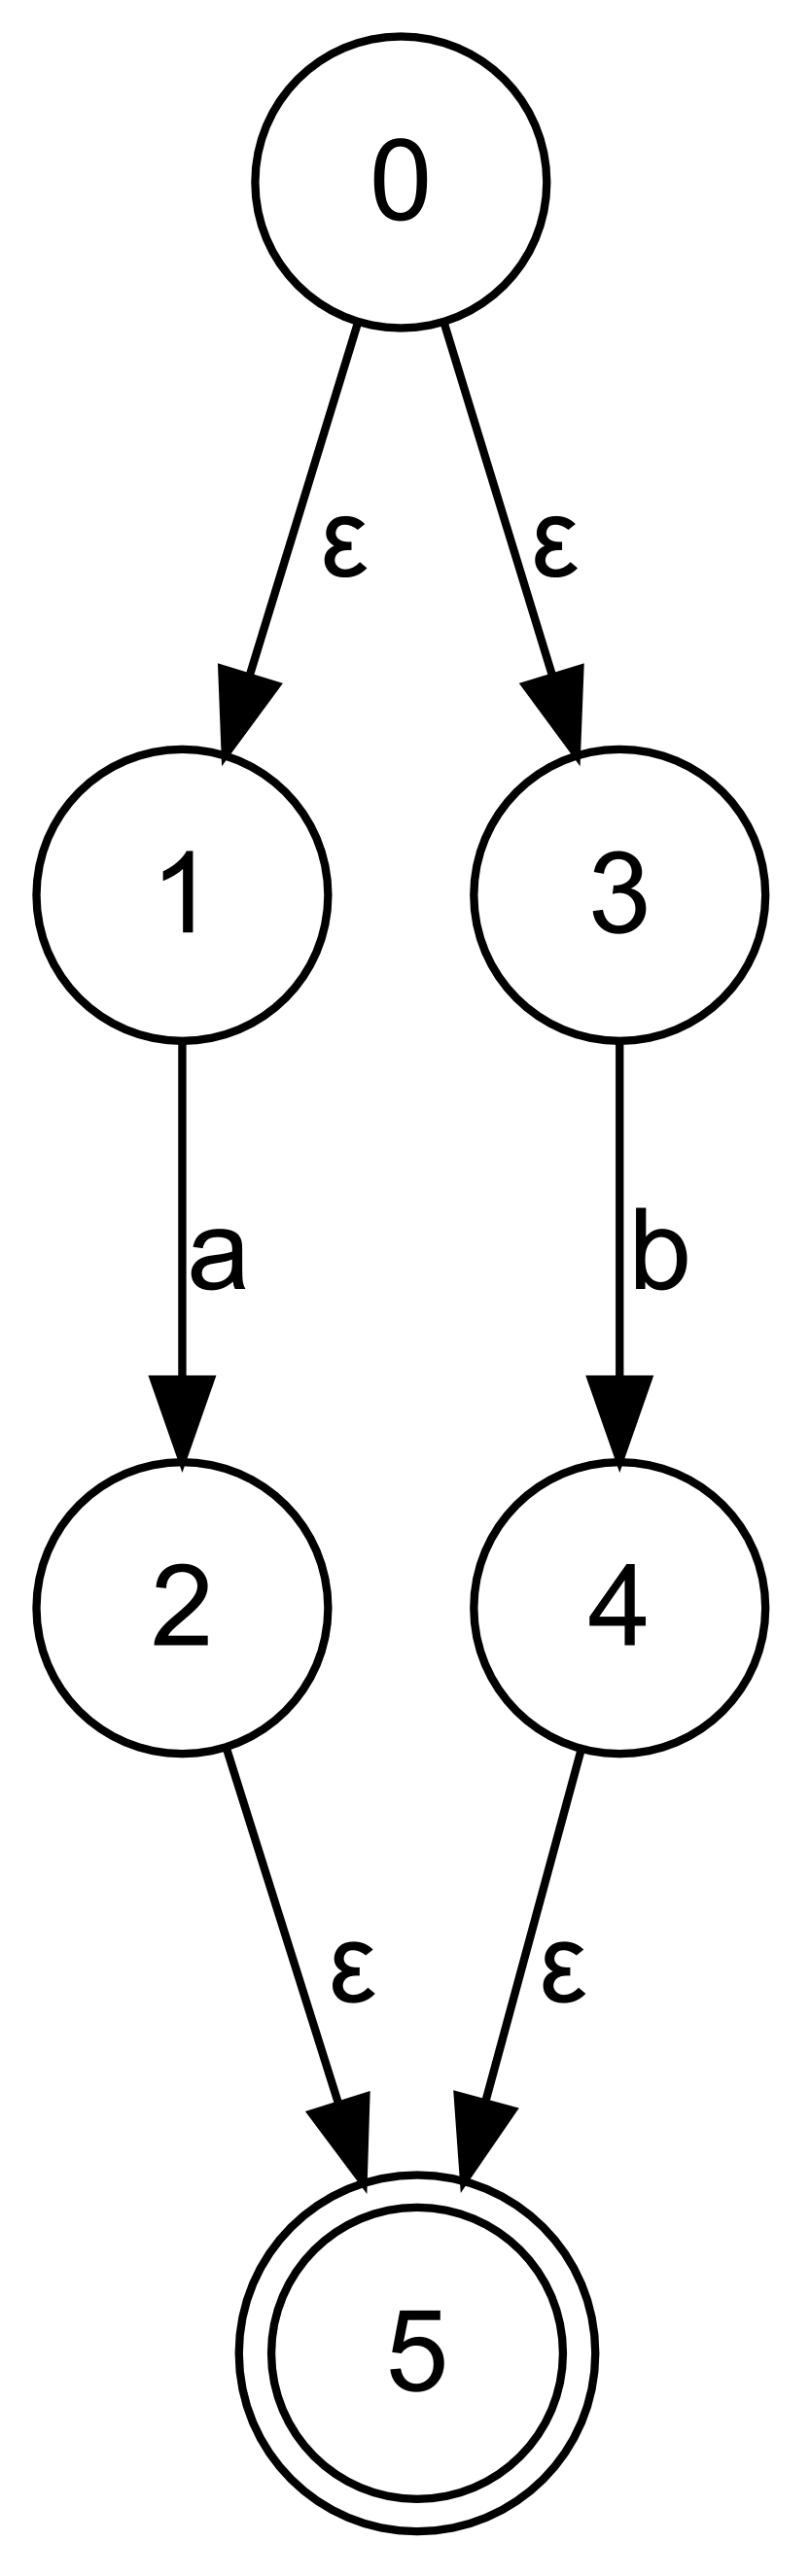
\includegraphics[width=0.2\textwidth]{lib/A_OR_B.png}
  \caption{NFA of the expression $a | b$}
\label{fig:A_OR_B}
\end{figure}

Once a NFA-structure has been build, we can start match a text against the NFA, looking for a match. We do this by having a list of states, each state looks at a node of the structure, and counts the number of previous hits which lead to the current state. Whenever a new character is being parsed from the text file, each state is asked to look at its node, and determine if it's possible to accept the given character in the NFA, either by moving forward through a pointer labeled with the character in question, or alternatively by epsilon pointers, each epsilon making a new state similar to the original, which then looks at its pointers for the character being parsed. If any of these match then the state moves on onto the matching pointer's node and the hit counter is incremented. %Alternatively the state will be dropped as it no longer matches the parsed string.

\begin{figure}[h!]
\begin{minipage}[b]{0.45\linewidth}
  \centering
      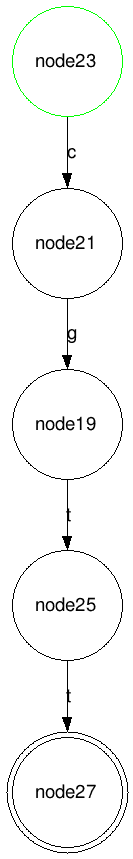
\includegraphics[width=0.2\textwidth]{lib/cgtt1.png}
    \caption{NFA of $CGTT$, with a state looking at node23 and a counter of $N$.\\}
    \label{fig:CGTT_1}
  \end{minipage}
\begin{minipage}[b]{0.45\linewidth}
\centering
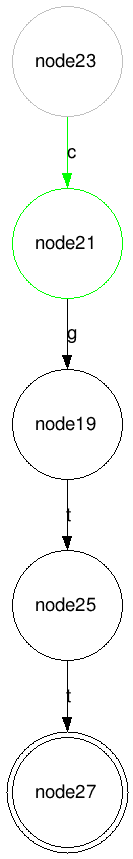
\includegraphics[width=0.2\textwidth]{lib/cgtt2.png}
 \caption{Next iteration of the state on Figure~\ref{fig:CGTT_1}, the state is now in node21, and the counter was incremented, to being $N+1$.}
    \end{minipage}
\label{fig::cgtt}
\end{figure}

Whenever a state reaches the ending node of the NFA, the number of matches that lead to the end node is returned, allowing for printing of the matched string, and the state is done. If no transition is possible in a state, it does not match the parsed character it is done, and it deleted.

For each new character being parsed, a new state is being added to the states in the code, this state will have a matching counter of 0, and will look at the start of the NFA, allowing new matches to be made.

\subsubsection{Insertions, Deletions and Mutations}
Currently our implementation supports a simple solution to the insertion, deletion and mutation problem, which is achieved by having a counter for insertions, deletions and mutation in each state, these counters symbolise the number of allowed occurrences of each mutation, insertion and deletion.
Whenever a match is not possible in parsing a file, if insertions is allowed, the match counter will be incremented, but the state won't move from its current node.
If deletions are allowed, match counter is left unchanged, and the state will move on to the node pointed to in the unmatched pointer.
If mutations are allowed, the same happens as in a deletion, but the counter is incremented. Figure~\ref{fig:ins_mut_del} illustrates how states move through a NFA when mismatches occur. 

\begin{figure}[h!]
  \centering
      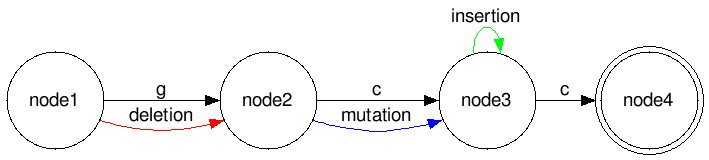
\includegraphics[width=0.6\textwidth]{lib/gcc_ins_mut_del.png}
  \caption{Simple NFA of $GCC$, showing behaviour of insertion, mutation and deletion}
\label{fig:ins_mut_del}
\end{figure}
Depending on the number of insertions, deletions and mutations allowed, this approach will grant each state a much longer lifespan, and for each non-matching character parsed, one state may turn into three, which all needs to be processed for each new character parsed, resulting in an increasingly slower running time as the allowed number of insertions, deletions and mutations increase, but it does give us the utility that we require.
\label{state:insertion1}


%In the next iteration of our implementation, we aim to implement levenstein automations\cite{WikiLevenshtein}, which hopefully will help speed up the runtime, and also, currently our solution will work on any given regular expression, thus a logical step which also may deliver some increase in performance would be to enforce a constriction such that it only allows for a RNA language similar to that defined in Section~\ref{section:RE}.

\subsection{Experimental Results \& Tests} % HAUGAARD
While no extensive benchmarking has been made yet, we did time the running time of our own implementation versus that of scan\_for\_matches and TRE (TRE running through a file with all newlines trimmed, to bypass the problem with returning after each delimiter).

Searching for pattern $GGAGTGCAAGCGTT$ with 1 insertion, 11 times each on a 40MB, 80MB and a 194MB file, we got the following average running times (in seconds):\\
\begin{tabular}{ c | c | c |  c }
 &scan\_for\_matches & TRE & Our C++ \\
 \hline
 40MB & 2.2 & 13.6 & 22.0 \\
 80MB & 4.4 & 27.8 & 45.2 \\
 194MB & 12.2 &  71.3 &  114.6
\end{tabular}

To verify the statement made in Section \ref{state:insertion1} about insertions, mutations and deletions increasing the runtime, running the same search, but without any insertions allowed, on the 194MB file we got the following running times, on an average over 11 runs.\\
\begin{tabular}{ c | c | c |  c }
 &scan\_for\_matches & TRE & Our C++ \\
 \hline
 194MB & 4.6 &  10.6 &  65.1
\end{tabular}

Showing that, our implementation is by far the slowest, not yet being a viable alternative to scan\_for\_matches, the same could be said about TRE, although it has a much more acceptable running-time.
